\section{最坏值函数}
\label{sec:minimax-value-function}

外层真正面对的目标是什么？本节把内层收进一个只依赖$\bm{x}$的函数，然后研究这个函数的性质，因为外层能用什么算法，全由这些性质决定。

\begin{definition}[最坏值函数]
\label{def:minimax-value}
称
\begin{equation}
 \phi(\bm{x})=\sup_{\bm{y}\in\bm{Y}}f(\bm{x},\bm{y})
 \label{eq:minimax-value}
\end{equation}
为\term{最坏值函数}（worst-case value function），它在某些点上可以取$+\infty$。上确界能够达到时，记最优响应的集合为
\begin{equation}
 \bm{Y}^\star(\bm{x})=\{\bm{y}\in\bm{Y}:f(\bm{x},\bm{y})=\phi(\bm{x})\}.
 \label{eq:minimax-response-set}
\end{equation}
\end{definition}

问题~\eqref{eq:minimax-problem}于是成为普通的单层问题$\inf_{\bm{x}\in\bm{X}}\phi(\bm{x})$。难点全部转移到了$\phi$上：它的每个函数值都要解一次最大化，它未必处处有限，也未必光滑。

有一点性质不需要任何计算。若对每个$\bm{y}\in\bm{Y}$，$f(\cdot,\bm{y})$都是凸函数，则$\phi$是凸函数，因为对任意$\theta\in[0,1]$，
\[
 f(\theta\bm{x}_1+(1-\theta)\bm{x}_2,\bm{y})\leq\theta f(\bm{x}_1,\bm{y})+(1-\theta)f(\bm{x}_2,\bm{y})\leq\theta\phi(\bm{x}_1)+(1-\theta)\phi(\bm{x}_2),
\]
再对$\bm{y}$取上确界即可。这里对$\bm{y}$一侧没有任何要求，$(x-y)^2$关于$y$是凸的，$\phi$照样是凸的。

内层可能出现三种不同的状况，它们影响的事情也不同，见表~\ref{tab:minimax-three-levels}。

\begin{BookInlineTable}
 \centering
 \begin{tabular}{@{}lll@{}}
  \toprule
  内层的状况 & 影响什么 & 反例\\
  \midrule
  最坏值有限 & 问题在该$\bm{x}$处是否有意义 & $f=xy$，$Y=\mathbb{R}$\\
  上确界达到 & 内层能否解出一个响应 & $f=x^2-e^{-y}$，$Y=\mathbb{R}$\\
  最优响应唯一 & 外层是否可微 & $f=xy$，$Y=[-1,1]$，$x=0$\\
  \bottomrule
 \end{tabular}
 \caption{内层的三种状况及其影响。反例说明相应性质可能失败。}
 \label{tab:minimax-three-levels}
\end{BookInlineTable}

第一行里，$x\neq0$时$\sup_{y\in\mathbb{R}}xy=+\infty$，只有$x=0$处最坏值有限。第二行里$\phi(x)=x^2$有限，但$-e^{-y}$在$y\to+\infty$时只是趋于$0$，没有哪个$y$达到上确界，内层的算法会一直往无穷远走。第三行里$x=0$时$f\equiv0$，每个$y$都是最优响应。

\subsection{响应切换}
\label{sec:minimax-switch}

光滑的$f$是否给出光滑的$\phi$？最简单的例子已经说明不会。取$f(x,y)=xy$，$Y=[-1,1]$。$f$关于$y$线性，最大值在端点，于是
\begin{equation}
 \phi(x)=\max\{x,-x\}=\lvert x\rvert.
 \label{eq:minimax-abs}
\end{equation}

每条直线$f(\cdot,y)$都光滑，它们的上边缘在原点却有折角，见图~\ref{fig:minimax-response-switch}(a)。原因是起作用的响应在$x=0$处换了人：$x>0$时最优响应是$y=1$，$x<0$时是$y=-1$。外层目标的尖点，正是内层最优响应切换的地方。这个切换与第~\ref{chap:nonsmooth-composite-optimization}章有限个函数取最大值时活跃分支的交替是同一个机制，只是这里的分支可能有无穷多条。

\begin{BookInlineFigure}
 \centering
 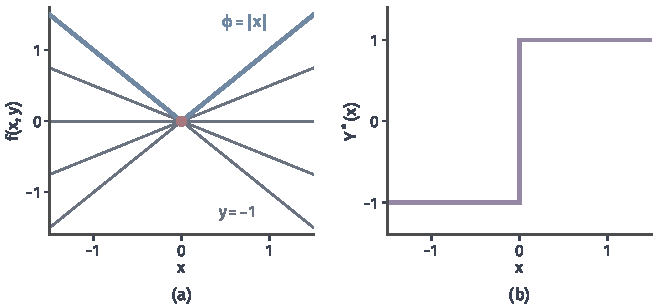
\includegraphics[width=112mm]{figures/05-optimization/07-multiple-criteria-and-nested-optimization/matplotlib/minimax-response-switch/figure.pdf}
 \caption{$f(x,y)=xy$，$Y=[-1,1]$。(a)灰线是$y=0,\pm\frac12,\pm1$时的直线，蓝线是上边缘$\phi(x)=\lvert x\rvert$，红点是外层最优解。(b)紫线是最优响应集合$Y^\star(x)$的图像，在$x=0$处是一整条竖直线段。}
 \label{fig:minimax-response-switch}
\end{BookInlineFigure}

图~\ref{fig:minimax-response-switch}(b)画出了$Y^\star(x)$。在$x\neq0$处它是单点，在$x=0$处是整个区间，这说明最优响应应当看作集合值映射。$(x-y)^2$的情形更极端：$Y^\star(0)=\{-1,1\}$是两个分开的点，集合甚至不连通。

下面的定理给出响应集合紧时能够保证的全部好性质。它说明响应集合可以跳，但图像是闭的，$\phi$本身仍然连续。

\begin{theorem}[紧响应集上的最坏值函数]
\label{thm:minimax-compact}
设$\bm{Y}$非空且紧，$f$在$\bm{X}\times\bm{Y}$上连续。则
\begin{enumerate}
 \item 对每个$\bm{x}\in\bm{X}$，上确界达到，$\bm{Y}^\star(\bm{x})$非空且紧；
 \item $\phi$在$\bm{X}$上有限且连续；
 \item 若$\bm{x}_k\to\bm{x}$，$\bm{y}_k\in\bm{Y}^\star(\bm{x}_k)$，$\bm{y}_k\to\bar{\bm{y}}$，则$\bar{\bm{y}}\in\bm{Y}^\star(\bm{x})$。
\end{enumerate}
\end{theorem}

\begin{proof}
第一条。$f(\bm{x},\cdot)$是紧集上的连续函数，最大值存在。$\bm{Y}^\star(\bm{x})$是连续函数$f(\bm{x},\cdot)$的水平集，是紧集$\bm{Y}$的闭子集，所以紧。

第二条。设$\bm{x}_k\to\bm{x}$。集合$\bm{K}=\{\bm{x}_k\}\cup\{\bm{x}\}$是紧的，$f$在紧集$\bm{K}\times\bm{Y}$上一致连续。记
\[
 \delta_k=\max_{\bm{y}\in\bm{Y}}\lvert f(\bm{x}_k,\bm{y})-f(\bm{x},\bm{y})\rvert\to0.
\]
对任意$\bm{y}$，有
\[
 f(\bm{x}_k,\bm{y})\leq f(\bm{x},\bm{y})+\delta_k\leq\phi(\bm{x})+\delta_k.
\]
对$\bm{y}$取最大，得到$\phi(\bm{x}_k)\leq\phi(\bm{x})+\delta_k$。交换$\bm{x}_k$与$\bm{x}$的角色，得到$\phi(\bm{x})\leq\phi(\bm{x}_k)+\delta_k$。所以$\phi(\bm{x}_k)\to\phi(\bm{x})$。

第三条。由$\bm{y}_k$的最优性，$f(\bm{x}_k,\bm{y}_k)=\phi(\bm{x}_k)$。令$k\to\infty$，用$f$和$\phi$的连续性，得到$f(\bm{x},\bar{\bm{y}})=\phi(\bm{x})$。
\end{proof}

第三条对应图~\ref{fig:minimax-response-switch}(b)的形状：从左右两侧趋于$x=0$时响应趋于$\pm1$，这两个极限都落在$Y^\star(0)$里。反过来不成立，$Y^\star(0)$中的$y=\frac12$不是任何邻近点响应的极限，所以这个映射不是连续的。

\subsection{值函数导数}
\label{sec:minimax-danskin}

要用梯度类方法更新$\bm{x}$，需要$\phi$的导数，而$\phi$本身没有显式表达式。能不能不微分内层的解？

看图~\ref{fig:minimax-danskin}(a)。在$x=0.5$处，起作用的是$y=-1$这条抛物线，上边缘在这里与它相切。切线的斜率就是这条抛物线在$x=0.5$处关于$x$的导数。$y$本身随$x$怎样变，在一阶上不起作用，因为$y$已经处在最优位置，朝任何可行方向挪动，代价都不会一阶增加。

第~\ref{chap:parametric-sensitivity}章的Danskin型结果给出了精确的说法。那里研究固定集合$\bm{C}$上的最优值函数$V(\bm{\theta})$，把它用到$-f$上，记号换成本章的，就得到下面的结论，证明见该章。

\begin{theorem}[最坏值函数的方向导数]
\label{thm:minimax-danskin}
设$\bm{X}\subseteq\mathbb{R}^{n}$开，$\bm{Y}$非空且紧，$f$与$\nabla_{\bm{x}}f$在$\bm{X}\times\bm{Y}$上连续。则对每个$\bm{x}\in\bm{X}$和方向$\bm{d}$，
\begin{equation}
 \phi'(\bm{x};\bm{d})=\max_{\bm{y}\in\bm{Y}^\star(\bm{x})}\bigl\langle\nabla_{\bm{x}}f(\bm{x},\bm{y}),\bm{d}\bigr\rangle.
 \label{eq:minimax-danskin}
\end{equation}
若$\bm{Y}^\star(\bm{x})=\{\bm{y}^\star(\bm{x})\}$是单点，则$\phi$在$\bm{x}$处可微，且
\begin{equation}
 \nabla\phi(\bm{x})=\nabla_{\bm{x}}f(\bm{x},\bm{y}^\star(\bm{x})).
 \label{eq:minimax-danskin-gradient}
\end{equation}
\end{theorem}

式~\eqref{eq:minimax-danskin}取最大值，是因为沿方向$\bm{d}$走一小步之后，起作用的是在这个方向上增长最快的那条响应。在开头的例子里，$\nabla_xf=2(x-y)$。$x=0.5$时响应唯一，$y^\star=-1$，式~\eqref{eq:minimax-danskin-gradient}给出
\[
 \phi'(0.5)=2(0.5+1)=3.
\]
它与直接求导$\phi'(x)=2(x+1)$的结果一致。

在$x=0$处，$Y^\star(0)=\{-1,1\}$，两个响应的偏导数是$2$和$-2$。式~\eqref{eq:minimax-danskin}给出
\[
 \phi'(0;d)=\max\{2d,-2d\}=2\lvert d\rvert.
\]
直接展开，得到
\[
 \phi(d)-\phi(0)=(\lvert d\rvert+1)^2-1=2\lvert d\rvert+d^2,
\]
一阶部分相同。

\begin{BookInlineFigure}
 \centering
 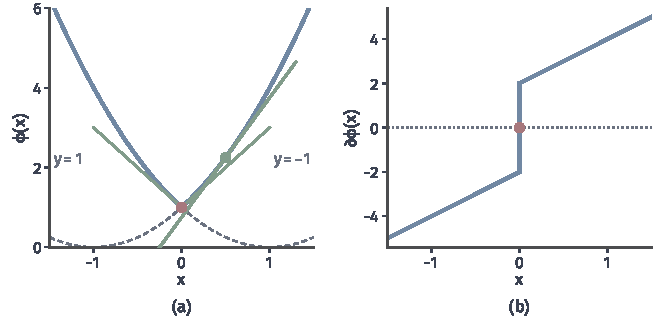
\includegraphics[width=112mm]{figures/05-optimization/07-multiple-criteria-and-nested-optimization/matplotlib/minimax-danskin/figure.pdf}
 \caption{$\phi(x)=(\lvert x\rvert+1)^2$的导数信息。(a)灰色虚线是$y=\pm1$两条抛物线，蓝线是上边缘。绿点$x=0.5$处只有一条活动响应，绿线是斜率为$3$的切线。红点$x=0$处两条响应同时活动，两段绿线的斜率是$\pm2$。(b)次微分的集值图像，在$x=0$处是竖直线段$[-2,2]$，它穿过点线$0$，说明$x=0$是最优解。}
 \label{fig:minimax-danskin}
\end{BookInlineFigure}

\paragraph{条件的作用}
定理要求响应集固定。这个条件去掉，公式就错了。取$f(x,y)=y$，让响应集随方案移动，$Y(x)=[-1,x]$，$x>-1$。则$\phi(x)=x$，导数是$1$，而$\partial f/\partial x\equiv0$。漏掉的部分来自集合边界的移动，要由乘子计入，这正是第~\ref{chap:parametric-sensitivity}章一般含参约束的内容。本章$\bm{Y}$不依赖$\bm{x}$，这个问题不出现。

紧性也不能省。$\bm{Y}$不紧时响应可能不存在，式~\eqref{eq:minimax-danskin}的右端失去意义，表~\ref{tab:minimax-three-levels}第二行就是这样。

\paragraph{关于$\bm{x}$凸时的次梯度集合}
多响应时只有方向导数还不够方便。若$f$关于$\bm{x}$凸，$\phi$是凸函数，可以用第~\ref{chap:nonsmooth-composite-optimization}章的次微分：$\bm{g}$是$\phi$在$\bm{x}$处的次梯度，指对所有$\bm{x}'$都有
\[
 \phi(\bm{x}')\geq\phi(\bm{x})+\langle\bm{g},\bm{x}'-\bm{x}\rangle.
\]

该章对有限个函数的最大值证明了次微分是活跃梯度的凸包，下面的定理把分支数推广到紧集上的无穷多个。

\begin{theorem}[最坏值函数的次微分]
\label{thm:minimax-subdiff}
设$\bm{X}=\mathbb{R}^{n}$，$\bm{Y}$非空且紧，$f$与$\nabla_{\bm{x}}f$连续，且对每个$\bm{y}\in\bm{Y}$，$f(\cdot,\bm{y})$是凸函数。则
\begin{equation}
 \partial\phi(\bm{x})=\operatorname{conv}\bigl\{\nabla_{\bm{x}}f(\bm{x},\bm{y}):\bm{y}\in\bm{Y}^\star(\bm{x})\bigr\}.
 \label{eq:minimax-subdiff}
\end{equation}
\end{theorem}

\begin{proof}
记右端为$\bm{K}$。$\bm{Y}^\star(\bm{x})$是紧集，它在连续映射$\nabla_{\bm{x}}f(\bm{x},\cdot)$下的像也是紧集，$\mathbb{R}^n$中紧集的凸包仍是紧集，所以$\bm{K}$紧且凸。

先证$\bm{K}\subseteq\partial\phi(\bm{x})$。任取$\bm{y}\in\bm{Y}^\star(\bm{x})$和$\bm{x}'$。由$\phi$的定义和$f(\cdot,\bm{y})$的凸性，
\[
 \phi(\bm{x}')\geq f(\bm{x}',\bm{y})\geq f(\bm{x},\bm{y})+\langle\nabla_{\bm{x}}f(\bm{x},\bm{y}),\bm{x}'-\bm{x}\rangle.
\]
左边第二项的$f(\bm{x},\bm{y})$等于$\phi(\bm{x})$。把这样的不等式按凸组合的权重相加，右端的向量就换成了$\bm{K}$中的任意元素。

再证反向。设$\bm{g}\in\partial\phi(\bm{x})$但$\bm{g}\notin\bm{K}$。$\bm{K}$非空、闭、凸，由第~\ref{chap:duality}章点与闭凸集的严格分离，存在$\bm{d}$，使
\[
 \langle\bm{g},\bm{d}\rangle>\max_{\bm{c}\in\bm{K}}\langle\bm{c},\bm{d}\rangle\geq\max_{\bm{y}\in\bm{Y}^\star(\bm{x})}\langle\nabla_{\bm{x}}f(\bm{x},\bm{y}),\bm{d}\rangle=\phi'(\bm{x};\bm{d}).
\]
最后的等号是式~\eqref{eq:minimax-danskin}。

另一方面，次梯度不等式给出
\[
 \phi(\bm{x}+s\bm{d})-\phi(\bm{x})\geq s\langle\bm{g},\bm{d}\rangle.
\]
除以$s>0$并令$s\downarrow0$，得到
\[
 \phi'(\bm{x};\bm{d})\geq\langle\bm{g},\bm{d}\rangle.
\]
这与上式矛盾。
\end{proof}

对开头的例子，活动偏导数是$\pm2$，所以$\partial\phi(0)=[-2,2]$，见图~\ref{fig:minimax-danskin}(b)。对$f=xy$，活动偏导数是$\lvert y\rvert\leq1$的全体$y$，所以$\partial\phi(0)=[-1,1]$。两者都含$0$，所以$x=0$都是全局最优解。

多响应时要注意一件事：只取其中一个响应，它给出的梯度未必是下降方向。在$(x-y)^2$的$x=0$处，取$y=1$，偏导数是$-2$，沿负偏导数方向是把$x$往正的方向移，而$\phi$沿这个方向是上升的。这和第~\ref{chap:nonsmooth-composite-optimization}章次梯度的负方向未必下降是同一回事。值函数的导数和次梯度只回答“外层目标对$\bm{x}$怎样变化”；$\bm{Y}$或约束也随参数变化时的完整敏感性，由第~\ref{chap:parametric-sensitivity}章处理。
